\subsection{Caso: \( D = 0.001 \)}


% T = 0
\subsubsection{Análise para o caso: \( D = 0.001 \) e \( t = 0 \)}

A Figura \ref{fig:advec_diffus_0.001_t0} mostra a distribuição da concentração de soluto no tempo inicial para um coeficiente de difusão \( D = 0.001 \). Neste caso, a diferença entre a advecção pura e a advecção-difusão é quase imperceptível, indicando que a influência da difusão é extremamente limitada neste estágio inicial. A forma retangular do perfil de concentração mantém-se praticamente inalterada, destacando o efeito mínimo da difusão quando \( D \) é substancialmente reduzido.

\begin{figure}[H]
    \centering
    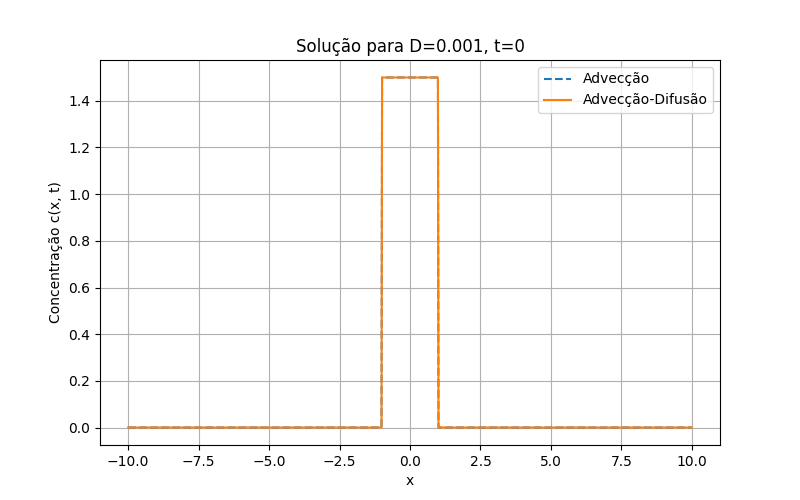
\includegraphics[width=0.7\textwidth]{code/plot/Advec_Difus_t0_D0.001.png}
    \caption{Comparação das soluções de advecção e advecção-difusão para \( D = 0.001 \) no tempo \( t = 0 \). A linha tracejada representa a advecção pura, enquanto a linha contínua, quase coincidente com a advecção pura, indica a advecção-difusão.}
    \label{fig:advec_diffus_0.001_t0}
\end{figure}

\begin{table}[H]
    \centering
    \caption{Valores numéricos da concentração para \( D = 0.001 \) e \( t = 0 \)}
    \begin{tabular}{ccc}
\toprule
x & Advecção & Advecção-Difusão \\
\midrule
-2.250000 & 0.000000 & 0.000000 \\
-1.690000 & 0.000000 & 0.000000 \\
-1.140000 & 0.000000 & 0.000000 \\
-0.580000 & 1.500000 & 1.500000 \\
-0.030000 & 1.500000 & 1.500000 \\
0.530000 & 1.500000 & 1.500000 \\
1.080000 & 0.000000 & 0.000000 \\
1.640000 & 0.000000 & 0.000000 \\
2.190000 & 0.000000 & 0.000000 \\
2.750000 & 0.000000 & 0.000000 \\
\bottomrule
\end{tabular}

\end{table}

% T = 1
\subsubsection{Análise para o caso: \( D = 0.001 \) e \( t = 1 \)}

A Figura \ref{fig:advec_diffus_0.001_t1} mostra a distribuição da concentração de soluto no tempo \( t = 1 \) para um coeficiente de difusão \( D = 0.001 \). Semelhante ao tempo \( t = 0 \), a difusão tem um efeito ainda muito limitado sobre a distribuição da concentração, que permanece praticamente idêntica à advecção pura. Isso demonstra que, para valores extremamente baixos de \( D \), a difusão é insuficiente para alterar significativamente o perfil inicial da concentração mesmo após um intervalo de tempo.

\begin{figure}[H]
    \centering
    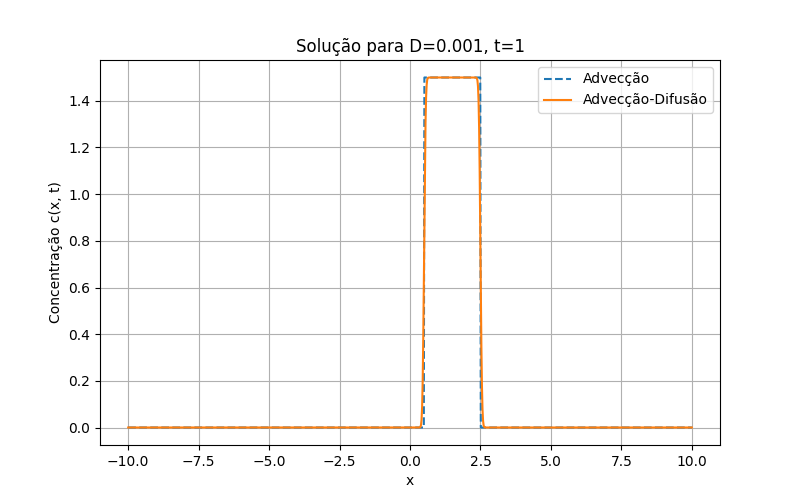
\includegraphics[width=0.7\textwidth]{code/plot/Advec_Difus_t1_D0.001.png}
    \caption{Comparação das soluções de advecção e advecção-difusão para \( D = 0.001 \) no tempo \( t = 1 \). A linha tracejada representa a advecção pura, enquanto a linha contínua, quase indistinguível, indica a advecção-difusão, evidenciando o efeito mínimo da difusão.}
    \label{fig:advec_diffus_0.001_t1}
\end{figure}

\begin{table}[H]
    \centering
    \caption{Valores numéricos da concentração para \( D = 0.001 \) e \( t = 1 \)}
    \begin{tabular}{ccc}
\toprule
x & Advecção & Advecção-Difusão \\
\midrule
-0.750000 & 0.000000 & 0.000000 \\
-0.190000 & 0.000000 & 0.000000 \\
0.360000 & 0.000000 & 0.001424 \\
0.920000 & 1.500000 & 1.500000 \\
1.470000 & 1.500000 & 1.500000 \\
2.030000 & 1.500000 & 1.500000 \\
2.580000 & 0.000000 & 0.046806 \\
3.140000 & 0.000000 & 0.000000 \\
3.690000 & 0.000000 & 0.000000 \\
4.250000 & 0.000000 & 0.000000 \\
\bottomrule
\end{tabular}

\end{table}


% T = 2
\subsubsection{Análise para o caso: \( D = 0.001 \) e \( t = 2 \)}

A Figura \ref{fig:advec_diffus_0.001_t2} mostra a distribuição da concentração de soluto no tempo \( t = 2 \) para um coeficiente de difusão \( D = 0.001 \). Neste momento, a diferença entre a advecção pura e a advecção-difusão continua sendo mínima, indicando que mesmo com o passar do tempo, a difusão com um coeficiente tão baixo não tem um impacto significativo na forma da distribuição da concentração. O perfil continua essencialmente retangular, destacando que a advecção domina o transporte do soluto.

\begin{figure}[H]
    \centering
    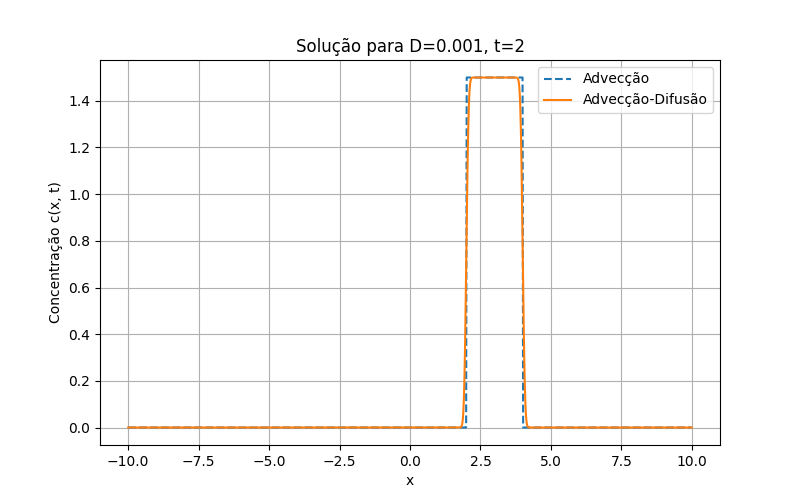
\includegraphics[width=0.7\textwidth]{code/plot/Advec_Difus_t2_D0.001.png}
    \caption{Comparação das soluções de advecção e advecção-difusão para \( D = 0.001 \) no tempo \( t = 2 \). A linha tracejada representa a advecção pura, enquanto a linha contínua, quase indistinguível da advecção, mostra o efeito ainda limitado da difusão.}
    \label{fig:advec_diffus_0.001_t2}
\end{figure}

\begin{table}[H]
    \centering
    \caption{Valores numéricos da concentração para \( D = 0.001 \) e \( t = 2 \)}
    \begin{tabular}{ccc}
\toprule
x & Advecção & Advecção-Difusão \\
\midrule
0.750000 & 0.000000 & 0.000000 \\
1.310000 & 0.000000 & 0.000000 \\
1.860000 & 0.000000 & 0.021068 \\
2.420000 & 1.500000 & 1.500000 \\
2.970000 & 1.500000 & 1.500000 \\
3.530000 & 1.500000 & 1.500000 \\
4.080000 & 0.000000 & 0.140724 \\
4.640000 & 0.000000 & 0.000000 \\
5.190000 & 0.000000 & 0.000000 \\
5.750000 & 0.000000 & 0.000000 \\
\bottomrule
\end{tabular}

\end{table}

% T = 3
\subsubsection{Análise para o caso: \( D = 0.001 \) e \( t = 3 \)}

A Figura \ref{fig:advec_diffus_0.001_t3} mostra a distribuição da concentração de soluto no tempo \( t = 3 \) para um coeficiente de difusão \( D = 0.001 \). Neste ponto, a advecção pura e a advecção-difusão continuam a apresentar perfis praticamente idênticos, com o perfil de concentração mantendo a forma retangular, evidenciando o efeito mínimo da difusão neste coeficiente.

\begin{figure}[H]
    \centering
    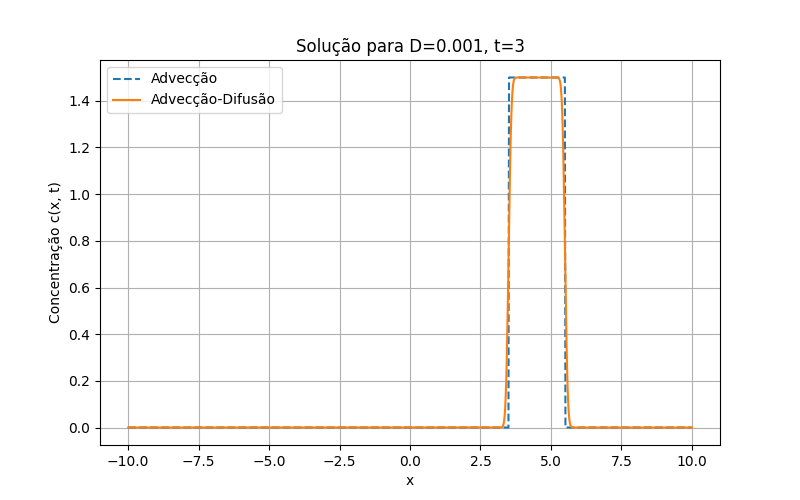
\includegraphics[width=0.7\textwidth]{code/plot/Advec_Difus_t3_D0.001.png}
    \caption{Comparação das soluções de advecção e advecção-difusão para \( D = 0.001 \) no tempo \( t = 3 \). A linha tracejada representa a advecção pura, enquanto a linha contínua, ainda quase indistinguível da advecção, ilustra a fraca influência da difusão.}
    \label{fig:advec_diffus_0.001_t3}
\end{figure}

\begin{table}[H]
    \centering
    \caption{Valores numéricos da concentração para \( D = 0.001 \) e \( t = 3 \)}
    \begin{tabular}{ccc}
\toprule
x & Advecção & Advecção-Difusão \\
\midrule
2.250000 & 0.000000 & 0.000000 \\
2.810000 & 0.000000 & 0.000000 \\
3.360000 & 0.000000 & 0.054724 \\
3.920000 & 1.500000 & 1.500000 \\
4.470000 & 1.500000 & 1.500000 \\
5.030000 & 1.500000 & 1.500000 \\
5.580000 & 0.000000 & 0.211503 \\
6.140000 & 0.000000 & 0.000000 \\
6.690000 & 0.000000 & 0.000000 \\
7.250000 & 0.000000 & 0.000000 \\
\bottomrule
\end{tabular}

\end{table}


% T = 4
\subsubsection{Análise para o caso: \( D = 0.001 \) e \( t = 4 \)}

A Figura \ref{fig:advec_diffus_0.001_t4} mostra a distribuição da concentração de soluto no tempo \( t = 4 \) para um coeficiente de difusão \( D = 0.001 \). Como nos momentos anteriores, a advecção pura e a advecção-difusão apresentam perfis quase idênticos, indicando que a difusão continua a ter um impacto muito limitado no perfil de concentração. Este padrão ressalta que, para coeficientes de difusão extremamente baixos como \( D = 0.001 \), a advecção domina predominantemente a dinâmica do transporte de soluto.

\begin{figure}[H]
    \centering
    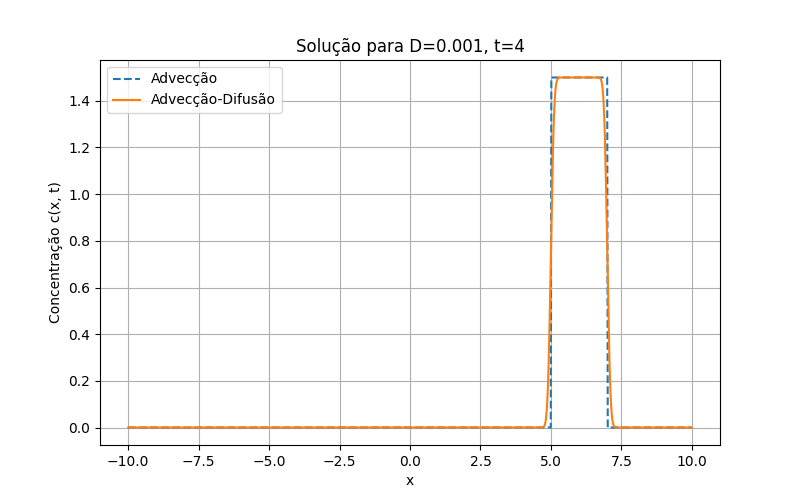
\includegraphics[width=0.7\textwidth]{code/plot/Advec_Difus_t4_D0.001.png}
    \caption{Comparação das soluções de advecção e advecção-difusão para \( D = 0.001 \) no tempo \( t = 4 \). A linha tracejada representa a advecção pura, enquanto a linha contínua, quase indistinguível, ilustra a falta de efeito significativo da difusão.}
    \label{fig:advec_diffus_0.001_t4}
\end{figure}

\begin{table}[H]
    \centering
    \caption{Valores numéricos da concentração para \( D = 0.001 \) e \( t = 4 \)}
    \begin{tabular}{ccc}
\toprule
x & Advecção & Advecção-Difusão \\
\midrule
3.750000 & 0.000000 & 0.000000 \\
4.310000 & 0.000000 & 0.000000 \\
4.860000 & 0.000000 & 0.090349 \\
5.420000 & 1.500000 & 1.499998 \\
5.970000 & 1.500000 & 1.500000 \\
6.530000 & 1.500000 & 1.500000 \\
7.080000 & 0.000000 & 0.263621 \\
7.640000 & 0.000000 & 0.000000 \\
8.190000 & 0.000000 & 0.000000 \\
8.750000 & 0.000000 & 0.000000 \\
\bottomrule
\end{tabular}

\end{table}


% T = 5
\subsubsection{Análise para o caso: \( D = 0.001 \) e \( t = 5 \)}

A Figura \ref{fig:advec_diffus_0.001_t5} mostra a distribuição da concentração de soluto no tempo \( t = 5 \) para um coeficiente de difusão \( D = 0.001 \). Como nos intervalos anteriores, a difusão continua a ter um impacto praticamente inexistente na forma da distribuição da concentração, com o perfil mantendo uma forma retangular quase idêntica à advecção pura. Esta consistência reforça a ideia de que, com valores extremamente baixos de \( D \), a difusão é insuficiente para alterar o perfil de concentração de maneira significativa ao longo do tempo observado.

\begin{figure}[H]
    \centering
    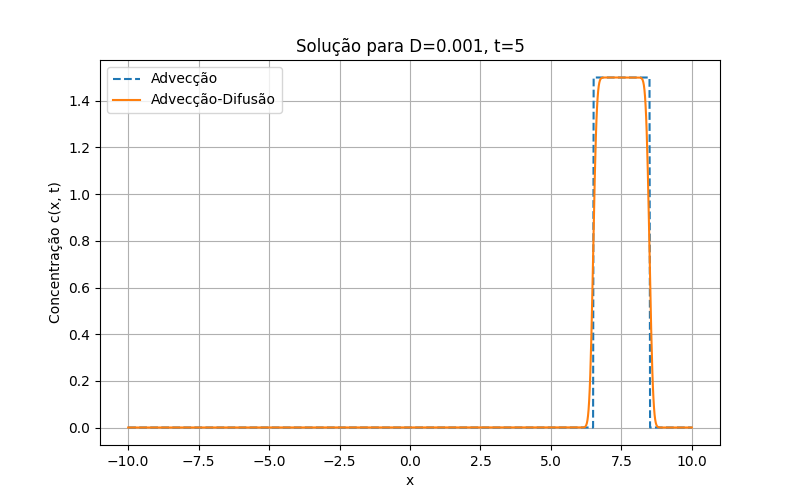
\includegraphics[width=0.7\textwidth]{code/plot/Advec_Difus_t5_D0.001.png}
    \caption{Comparação das soluções de advecção e advecção-difusão para \( D = 0.001 \) no tempo \( t = 5 \). A linha tracejada representa a advecção pura, enquanto a linha contínua, quase indistinguível, continua a mostrar o efeito mínimo da difusão.}
    \label{fig:advec_diffus_0.001_t5}
\end{figure}

\begin{table}[H]
    \centering
    \caption{Valores numéricos da concentração para \( D = 0.001 \) e \( t = 5 \)}
    \begin{tabular}{ccc}
\toprule
x & Advecção & Advecção-Difusão \\
\midrule
5.250000 & 0.000000 & 0.000000 \\
5.810000 & 0.000000 & 0.000000 \\
6.360000 & 0.000000 & 0.123650 \\
6.920000 & 1.500000 & 1.499977 \\
7.470000 & 1.500000 & 1.500000 \\
8.030000 & 1.500000 & 1.499998 \\
8.580000 & 0.000000 & 0.303493 \\
9.140000 & 0.000000 & 0.000000 \\
9.690000 & 0.000000 & 0.000000 \\
10.250000 & 0.000000 & 0.000000 \\
\bottomrule
\end{tabular}

\end{table}


% Conclusão do Caso
\subsection{Conclusão do Caso: \( D = 0.001 \)}
Durante o período observado de \( t = 0 \) a \( t = 5 \), as soluções numéricas para a equação de advecção-difusão com \( D = 0.001 \) apresentaram uma distribuição de concentração muito estável. Desde o início até o final do período estudado, advecção pura e advecção-difusão mostraram perfis quase idênticos, refletindo um impacto mínimo da difusão na evolução do soluto.

A persistência do perfil retangular indica que a difusão, neste nível baixo, não modifica significativamente a dinâmica do transporte de soluto, dominada pela advecção. A análise reforça que, embora a difusão possa ser impactante em coeficientes maiores, ela se torna quase irrelevante em valores tão baixos como \( D = 0.001 \), destacando a necessidade de ajustar cuidadosamente os parâmetros em modelos de advecção-difusão para simular corretamente os sistemas de transporte.
